\documentclass[11pt]{article}
\usepackage[margin=1in]{geometry}
\usepackage[T1]{fontenc}
\usepackage{lmodern}
\usepackage{graphicx}
\usepackage{amsmath}
\usepackage{booktabs}
\usepackage{caption}
\usepackage[colorlinks=true,linkcolor=blue,citecolor=blue,urlcolor=blue]{hyperref}
\graphicspath{{../figures/}}
\captionsetup{font=small}
\setlength{\parskip}{4pt}

\title{Does Drifting Channel Noise Help an Eavesdropper Hide in the BB84 Protocol?}
\author{Siddharth Boora}
\date{November 2026}

\begin{document}
\maketitle

\begin{abstract}
In the BB84 quantum key distribution protocol, Alice and Bob check for an eavesdropper (Eve) by measuring the error rate of a sample of their bits and stopping if it is above 11\%. Eve can try to hide by attacking only some of the qubits, so that their errors blend in with the channel's normal noise. Most analyses assume this noise stays constant, but in real systems it drifts up and down over time. I simulated BB84 with drifting noise and with steady noise at the same average, for rounds of 1024, 2048 and 4096 qubits, and measured how much an intercept-resend eavesdropper can get away with. I found that drift does not always help Eve. When the channel is fairly clean, drift actually makes them easier to catch, because they cannot predict sudden noise increases. Drift only starts to help them when the average noise is above about 6--7.5\%, depending on the number of qubits per round.
\end{abstract}

\section{Introduction}

BB84~\cite{BB84} lets two people, Alice and Bob, create a shared secret key using qubits (in real hardware, usually single photons of light). Each qubit is prepared in one of two random bases, Z or X. If an eavesdropper, Eve, measures a qubit in the wrong basis, they disturb it, which shows up as errors in Bob's results. To detect them, Alice and Bob publicly compare a random sample of their bits and calculate the quantum bit error rate (QBER). If the QBER is above a threshold they throw the key away. A common threshold is 11\%, which comes from the Shor--Preskill security proof~\cite{ShorPreskill}.

The problem is that Eve is not the only source of errors. Real channels are noisy, so Bob sees some errors even when nobody is listening. This gives Eve room to hide: if they attack only a fraction $f$ of the qubits, the extra errors they add might stay under 11\%. Earlier analyses of partial intercept-resend attacks, such as those by Fiorini \emph{et al.}~\cite{Fiorini24,Fiorini26}, treat the channel noise as a fixed number. In practice it changes over time because of temperature, vibration and the need to recalibrate equipment~\cite{YuanShields,PRTS}. A recent paper by Mordarski \emph{et al.}~\cite{Mordarski} modelled this kind of drifting noise and studied attacks found by machine learning.

Building on their noise model, this paper focuses on one specific question: \textbf{does drifting noise make it easier or harder for an intercept-resend eavesdropper to avoid detection, compared with steady noise of the same average level?} I also examined whether the answer depends on the number of qubits sent per round, since a smaller check sample gives a less precise estimate of the error rate.

Throughout this paper, 11\% is used as a fixed detection threshold. It is the asymptotic Shor--Preskill benchmark rather than a finite-key security threshold, which would be lower and would depend on the block size~\cite{Tomamichel}, so the results describe how often Eve passes this particular check.

\section{Method}

\subsection{The protocol and the check}

Each round, Alice sends $n$ qubits ($n = 1024$, 2048 or 4096). About half survive sifting (when Alice and Bob happened to use the same basis), and half of those are used for the check, so about $n/4$ bits are checked. If the error rate in this sample is above 11\%, the round is aborted, meaning Alice and Bob throw away its key. Because only a sample is checked, the measured error rate varies randomly from round to round.

\subsection{Eve's attack}

Eve uses intercept-resend on a fraction $f$ of the qubits: they measure each one in a random basis and send a new qubit with their result. Half the time they pick the wrong basis, and then Bob gets the wrong bit half the time, so they cause an error on $1/4$ of the bits they attack. If the channel itself flips bits with probability $e$, the expected error rate is
\begin{equation}
\text{QBER} = e + \frac{f}{4}(1-2e).
\end{equation}
Setting this equal to 11\% gives the largest fraction Eve can attack on average:
\begin{equation}
f_{\max} = \frac{4(0.11 - e)}{1 - 2e}.
\end{equation}

\subsection{Drifting noise}

Following Mordarski \emph{et al.}~\cite{Mordarski}, the noise level changes each round like this:
\begin{equation}
e_{t+1} = e_t + 0.1\,(\mu - e_t) + \sigma \cdot (\text{random normal number}),
\end{equation}
kept between 1\% and 30\%. This is called an Ornstein--Uhlenbeck process~\cite{OU}: the noise wanders randomly but is always pulled back toward its average $\mu$. I used $\sigma = 0.3\mu$, which matches their setting of $\mu = 10\%$, $\sigma = 0.03$. A session is 50 rounds. For comparison, the steady channel keeps the noise fixed at the same average. Figure~\ref{fig:drift} shows what this looks like.

\begin{figure}[tbp]
\centering
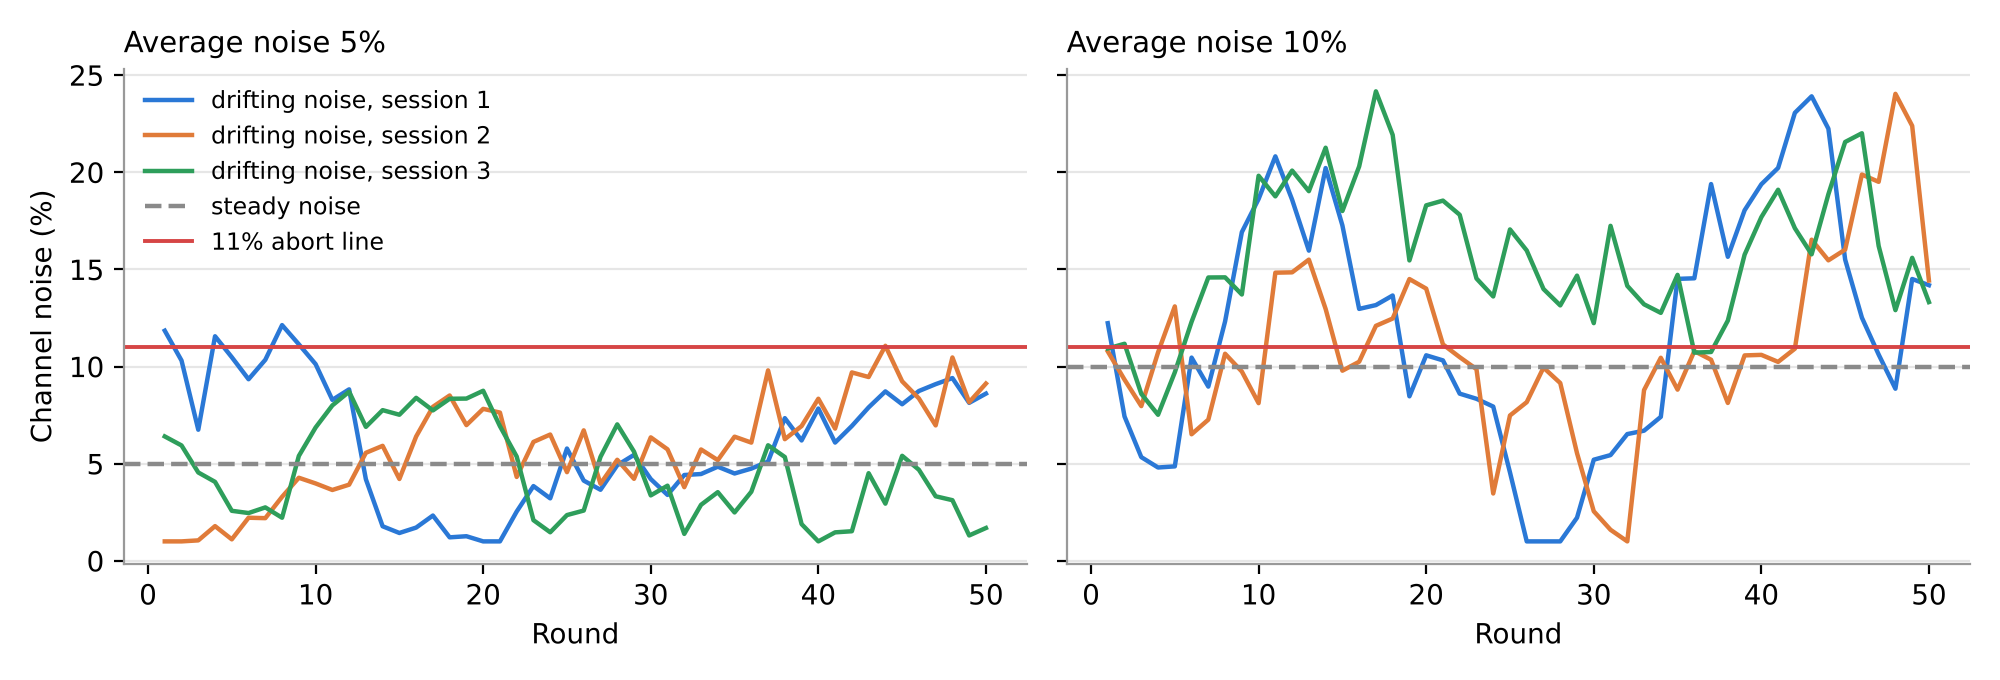
\includegraphics[width=0.95\textwidth]{fig1.png}
\caption{Three example sessions of drifting noise (blue, orange and green) compared with steady noise at the same average (grey dashed). The red line is the 11\% abort threshold.}
\label{fig:drift}
\end{figure}

\subsection{Eve's strategies}

I compared two strategies:
\begin{itemize}
\item \textbf{Fixed:} Eve attacks the same fraction $f$ every round.
\item \textbf{Adaptive:} after each round, Alice and Bob's error rate is public, so Eve can use it to estimate the current noise (Eve knows their own $f$, so they can subtract their part). They then pick the largest $f$ that gives them a chosen chance of passing the next check. Under drift this lets them attack more when the noise seems low.
\end{itemize}

\subsection{How I measured success}

If Eve attacks more, they get more information but also cause more aborted rounds, which Alice and Bob might notice. So I measured two things over thousands of simulated sessions:
\begin{itemize}
\item \textbf{Eve's information gain:} the percentage of all qubits that Eve read in rounds that were not aborted.
\item \textbf{Extra aborts:} how many more rounds were aborted with Eve present than without them.
\end{itemize}
I tried many attack strengths for each strategy. For the fixed Eve, the attack strength is the fraction $f$ of qubits they intercept, which I varied from 0.5\% to 45\%. For the adaptive Eve, it is the chance of passing the check that they aim for in each round, which I varied from 50\% to 99.9999\%. A higher target makes Eve more careful, so they intercept fewer qubits but are caught less often. For each strategy I report Eve's largest information gain among the attack strengths that cause at most 5 extra aborted rounds per 100. I also made sure the steady and drifting cases were compared at the same average noise.

\subsection{Code and checks}

The simulation is written in Python and was validated against the intercept-resend results of Rath \emph{et al.}~\cite{Rath}, giving a QBER of 2.52\% at $f = 0.1$ compared with the theoretical 2.5\%, and against Eq.~(1) with channel noise included. A smaller circuit-level version built in Qiskit~\cite{Qiskit}, with Eve measuring in the middle of the circuit, gave matching results. All code is at \url{https://github.com/siddharth-boora/bb84-research-paper}.

\section{Results}

\subsection{Even with steady noise, \texorpdfstring{$f_{\max}$}{f\_max} is not safe for Eve}

Figure~\ref{fig:steady} shows Eve's chance of passing the check with steady noise. At exactly $f_{\max}$ they only pass about half the time, because the measured error rate randomly lands above or below 11\%. To pass 90\% of the time they have to attack much less (Table~\ref{tab:steady}). Larger samples help them get closer to $f_{\max}$ because the measurement is less random.

\begin{figure}[tbp]
\centering
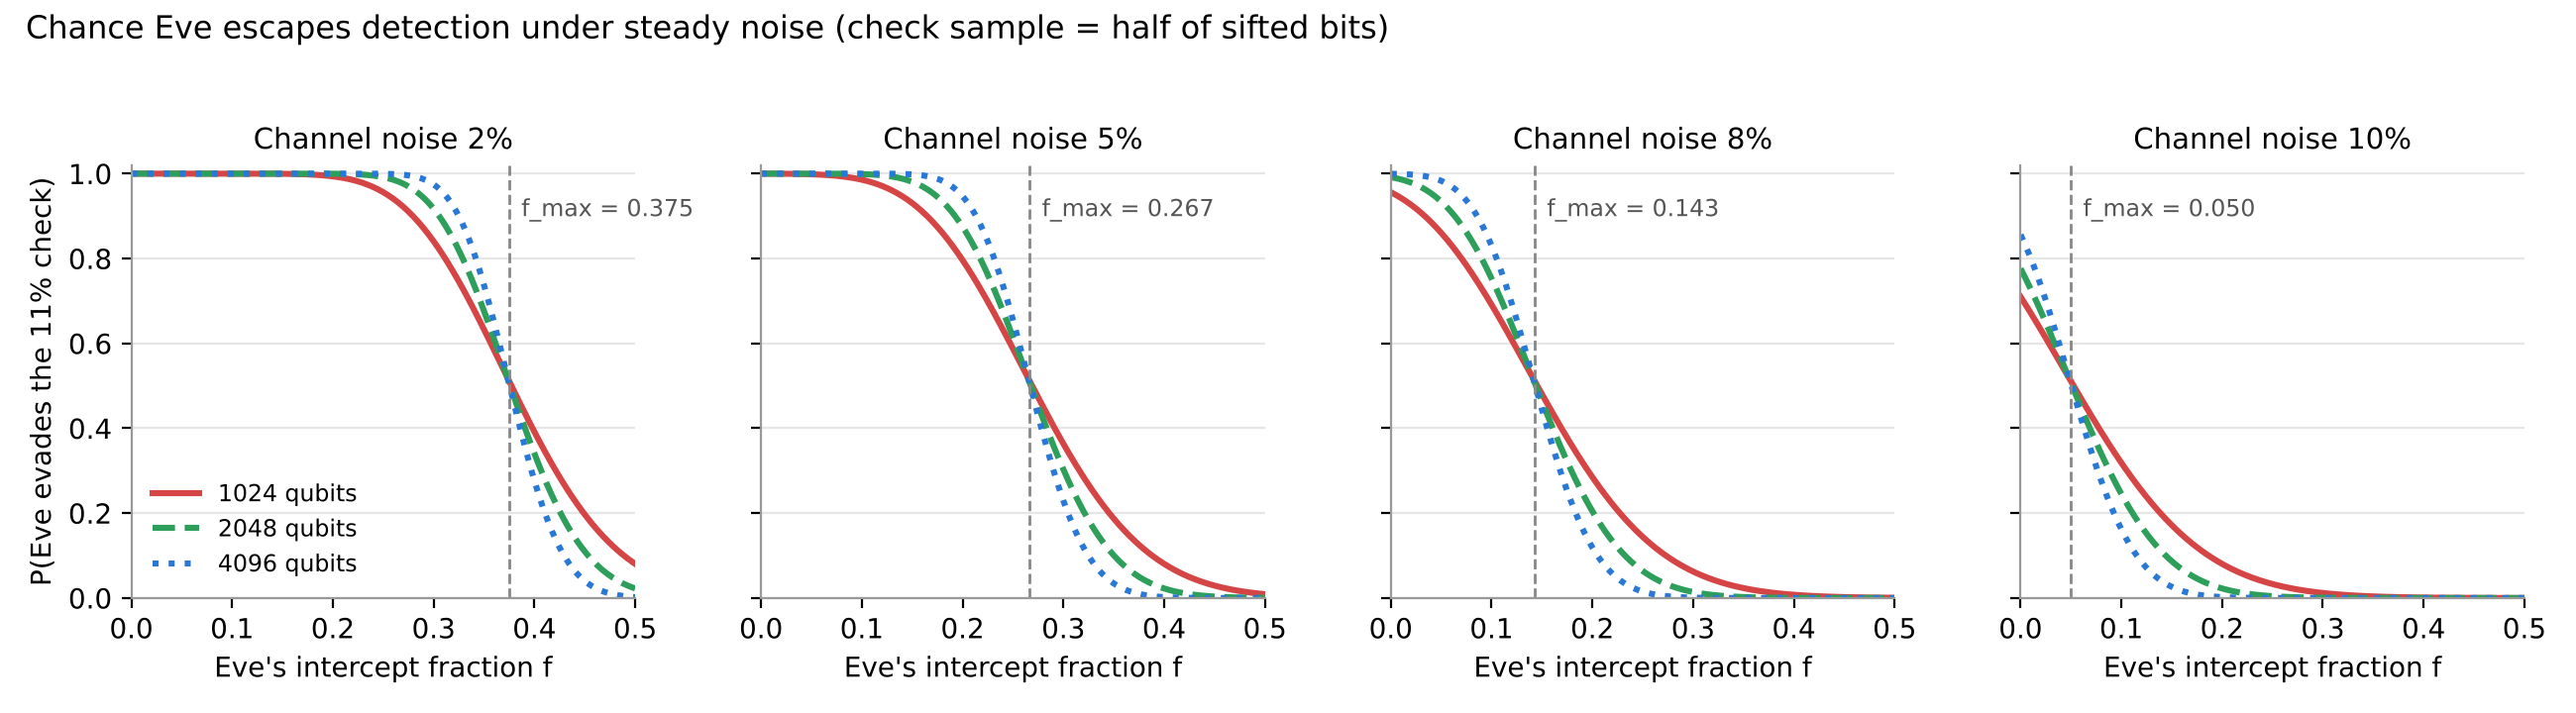
\includegraphics[width=\textwidth]{fig2.png}
\caption{Chance that Eve passes the 11\% check under steady noise, for different attack fractions $f$. The dashed line is $f_{\max}$.}
\label{fig:steady}
\end{figure}

\begin{table}[tbp]
\centering
\caption{Largest attack fraction that passes the check at least 90\% of the time (steady noise).}
\label{tab:steady}
\begin{tabular}{ccccc}
\toprule
Noise & $f_{\max}$ & 1024 qubits & 2048 qubits & 4096 qubits\\
\midrule
2\% & 0.375 & 0.280 & 0.306 & 0.325\\
5\% & 0.267 & 0.165 & 0.193 & 0.213\\
8\% & 0.143 & 0.034 & 0.063 & 0.086\\
10\% & 0.050 & 0 & 0 & 0\\
\bottomrule
\end{tabular}
\end{table}

\subsection{Drift can help or hurt Eve}

Figure~\ref{fig:n} compares Eve's information gain with steady and drifting noise at two average noise levels.

At \textbf{5\% average noise} (left), Eve does best with steady noise. With drift, even the adaptive Eve gets less (8.5--11.7\% instead of 11.2--17.0\%). The noise sometimes jumps up without warning, and if Eve is attacking at that moment the error rate goes over 11\% and their round is aborted.

At \textbf{10\% average noise} (right), it is the opposite. With steady noise, the channel is already so close to 11\% that Eve can barely attack at all (under 1\%). With drift, there are stretches where the noise drops, and the adaptive Eve uses them to get 3.6--4.0\%. Bigger samples make this gap grow: with steady noise their information gain shrinks as $n$ increases, but with drift it grows.

\begin{figure}[tbp]
\centering
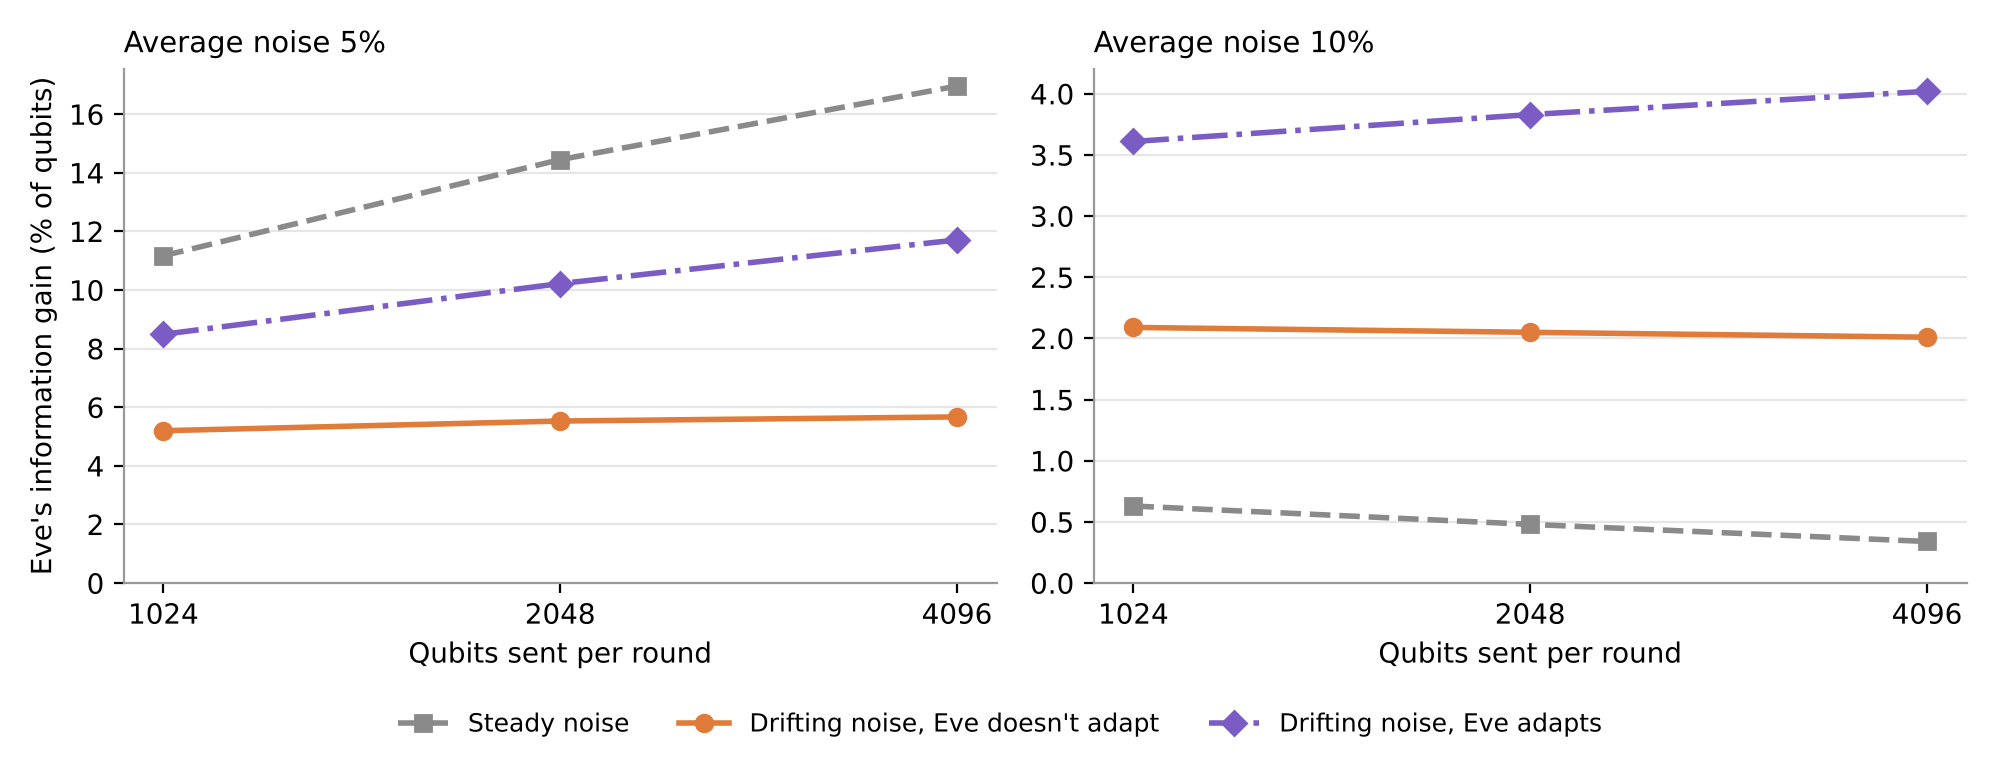
\includegraphics[width=0.95\textwidth]{fig3.png}
\caption{Eve's information gain (allowing at most 5 extra aborted rounds per 100) for steady and drifting noise.}
\label{fig:n}
\end{figure}

\subsection{Where drift switches from hurting to helping Eve}

To find the switching point, I repeated the comparison for average noise levels from 4.5\% to 10\% for the adaptive Eve. I ran the whole experiment 5 times with different random seeds to see how much the answer changes by chance. Each run simulates 1,500 sessions of 50 rounds at every noise level and qubit count, with new random noise, qubits, and check samples each time. Figure~\ref{fig:cross} shows the result: below zero, drift hurts Eve; above zero, it helps them.

\begin{figure}[tbp]
\centering
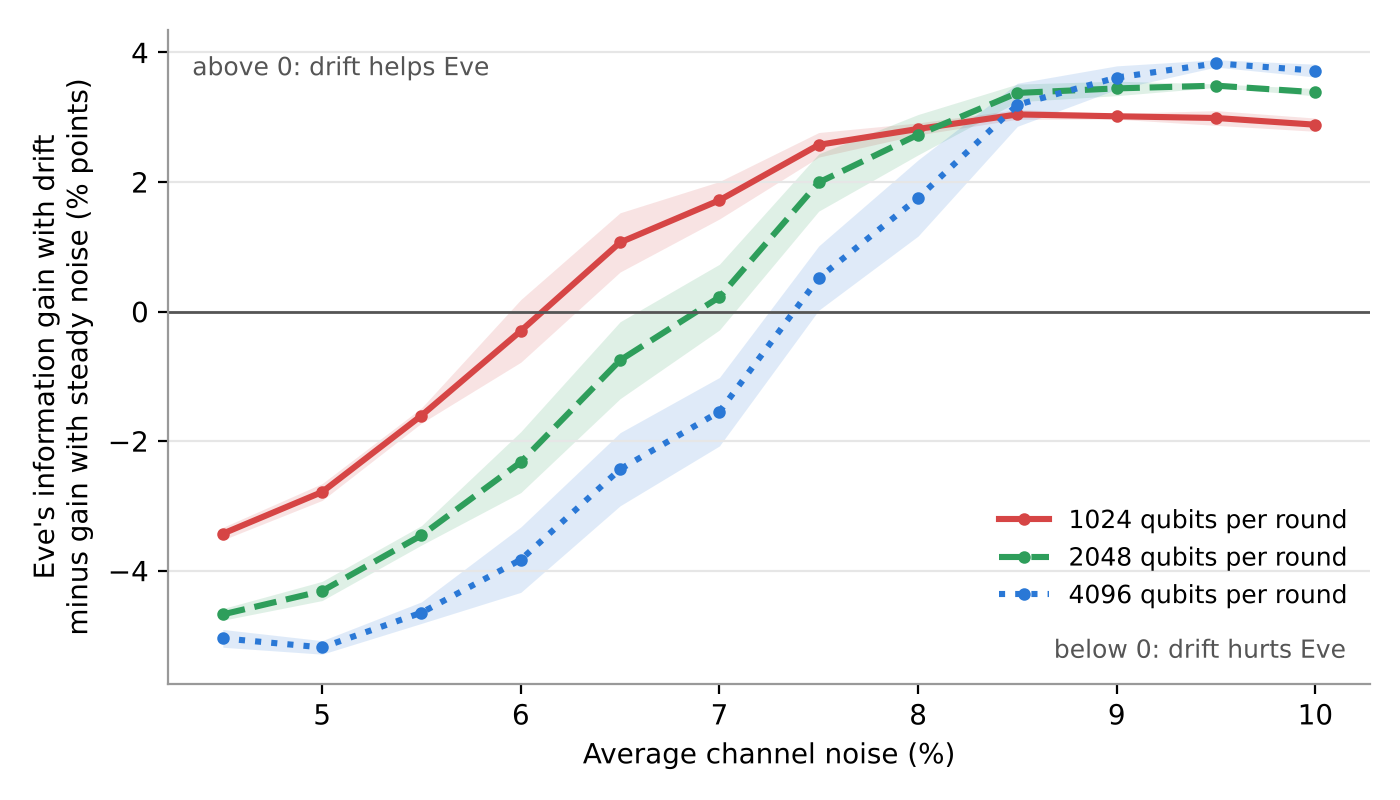
\includegraphics[width=0.75\textwidth]{fig4.png}
\caption{Adaptive Eve's information gain with drifting noise minus their information gain with steady noise. Shaded bands are 95\% confidence intervals from 5 independent runs.}
\label{fig:cross}
\end{figure}

\begin{table}[tbp]
\centering
\caption{Average noise level where drift starts to help the adaptive Eve (mean of 5 runs, with 95\% confidence interval).}
\label{tab:cross}
\begin{tabular}{lccc}
\toprule
 & 1024 qubits & 2048 qubits & 4096 qubits\\
\midrule
Crossover noise level & 6.1\% (6.0--6.3) & 6.9\% (6.8--7.0) & 7.4\% (7.3--7.5)\\
\bottomrule
\end{tabular}
\end{table}

The five runs agree closely: each crossover varies by only about 0.1 percentage points between runs, and Eve's information gain varies by at most about 0.2 percentage points, much smaller than the differences between steady and drifting noise. The crossover moves to higher noise as the number of qubits per round grows (Table~\ref{tab:cross}). So a larger check sample protects a wider range of channels from this effect.

\section{Discussion}

The main takeaway is that noisier, less stable channels help the attacker only near the threshold. On a fairly clean channel, drift works in Alice and Bob's favour, because an eavesdropper who plans their attack around the average noise gets caught when the noise suddenly rises. For someone running a QKD system, this suggests keeping the average error rate well below the crossover point, and that larger check samples help.

\textbf{Limitations.} This project has several simplifications:
\begin{itemize}
\item Eve only uses the basic intercept-resend attack. Real attackers could use stronger strategies, like the machine-learned attacks in Mordarski \emph{et al.}~\cite{Mordarski}.
\item Eve's information gain, as defined here, is a simple measure of how much Eve learns. A full security analysis would calculate the secret key rate using finite-key methods~\cite{Tomamichel}.
\item The channel model is simple (random bit flips only), with no photon loss or detector effects.
\item At 10\% average noise, about 45\% of rounds are aborted even without Eve, so that case is more of a stress test than a realistic link.
\item The results depend on the drift model. I briefly tested other noise patterns (no memory, sudden spikes, random walk); these results are in the code repository but not in this paper.
\end{itemize}

\section{Conclusion}

I simulated BB84 with drifting and steady channel noise to see whether drift helps an intercept-resend eavesdropper avoid the 11\% check. Drift hurts them on cleaner channels and helps them only when the average noise is above about 6--7.5\%, and this switching point rises with the number of qubits checked. In the future I would like to replace Eve's information gain with a real finite-key key-rate calculation and test stronger attacks.

\begin{thebibliography}{99}
\small
\bibitem{BB84} C.~H. Bennett and G. Brassard, ``Quantum cryptography: public key distribution and coin tossing,'' \emph{Proc. IEEE Int. Conf. on Computers, Systems and Signal Processing}, Bangalore, p.~175 (1984); reprinted in \emph{Theor. Comput. Sci.} \textbf{560}, 7 (2014).

\bibitem{ShorPreskill} P.~W. Shor and J. Preskill, ``Simple proof of security of the BB84 quantum key distribution protocol,'' \emph{Phys. Rev. Lett.} \textbf{85}, 441 (2000).

\bibitem{Tomamichel} M. Tomamichel, C.~C.~W. Lim, N. Gisin, and R. Renner, ``Tight finite-key analysis for quantum cryptography,'' \emph{Nat. Commun.} \textbf{3}, 634 (2012).

\bibitem{Mordarski} M. Mordarski, B. Gras, A. Shehata, D. Budina, and R. Bondesan, ``Learnt attacks on quantum key distribution under channel noise and device drift,'' preprint, \href{https://arxiv.org/abs/2610.01792}{arXiv:2610.01792} (2026).

\bibitem{Fiorini24} F. Fiorini, M. Pagano, R.~G. Garroppo, and A. Osele, ``Estimating interception density in the BB84 protocol: a study with a noisy quantum simulator,'' \emph{Future Internet} \textbf{16}, 275 (2024).

\bibitem{Fiorini26} F. Fiorini, R.~G. Garroppo, and M. Pagano, ``Threshold-based eavesdropper detection for partial intercept-resend attack in noisy BB84 quantum key distribution,'' \emph{Computer Networks} (2026).

\bibitem{YuanShields} Z.~L. Yuan and A.~J. Shields, ``Continuous operation of a one-way quantum key distribution system over installed telecom fibre,'' \emph{Opt. Express} \textbf{13}, 660 (2005).

\bibitem{PRTS} W. Wang, F. Xu, and H.-K. Lo, ``Prefixed-threshold real-time selection method in free-space quantum key distribution,'' \emph{Phys. Rev. A} \textbf{97}, 032337 (2018).

\bibitem{Rath} J. Rath, P. Panth, and P.~S.~N. Bhaskar, ``Quantum bit error rate analysis in BB84 quantum key distribution: measurement, statistical estimation, and eavesdropping detection,'' preprint, \href{https://arxiv.org/abs/2603.27278}{arXiv:2603.27278} (2026).

\bibitem{OU} G.~E. Uhlenbeck and L.~S. Ornstein, ``On the theory of the Brownian motion,'' \emph{Phys. Rev.} \textbf{36}, 823 (1930).

\bibitem{Qiskit} A. Javadi-Abhari \emph{et al.}, ``Quantum computing with Qiskit,'' preprint, \href{https://arxiv.org/abs/2405.08810}{arXiv:2405.08810} (2024).
\end{thebibliography}

\end{document}
